\chapter{Multiple Drift Detector} \label{chapt:MDD}

In this chapter we introduce multiple drift detector (MDD), a framework early detection of multiple types of concept drift. Section \ref{mdd:motivation} discusses the motivation for MDD. Section \ref{mdd:setting} describes the setting of MDD. Section \ref{mdd:code} provides pseudocode for MDD. Section \ref{mdd:graphics} introduces a graphical interface for MDD. Section \ref{mdd:illustration} illustrates the utility of MDD for our motivating example. Section \ref{mdd:conclusion} summarises this chapter and discusses future work.

%-------------------------------------------------------------------
% MOTIVATION
%-------------------------------------------------------------------

\section{Motivation} \label{mdd:motivation}

Existing drift detectors typically take the following approach. The time series of one or more performance metrics is monitored, and if a decline in the mean or rate of metric can be detected, then drift is signalled. The most common metric is accuracy \cite{DDM}\cite{EDDM}\cite{ADWIN}, although some detectors also use precision or recall \cite{LFR}\cite{klinkenberg_renz}\cite{DDM-OCIb}. The rationale is that under stable conditions the performance of the model should either improve or remain steady, so a decline in performance must indicate concept drift has occurred.

We posit that in some applications, a better approach to concept drift detection is to not only monitor the time series of  performance metrics, but also the time series of feature values and labels. Multiple drift detection (MDD) achieves this via multiple instantiations of a drift detector to monitor for feature drift, label drift, and real drift.

The main benefit of this approach is it can provide an early warning of concept drift. Specifically, if {\it feature} drift occurs, a drift detector which is monitoring the feature time series can alert the user to this change before all the labels become available. The user will then have the opportunity of recalling the model if it will no longer be able to perform adequately under the new distribution. 

The second benefit of this approach is that it helps the user obtain a more complete picture of how the data stream is evolving. A drift detector which simply signals when one or more performance metrics has declined affords little interpretability. By monitoring each of precision, recall, accuracy, label frequencies, and feature values, the user can better understand what exactly is driving a decline in model performance and how the decline is manifesting. This can help the user in choosing a dataset for model retraining. 

% There is a standard ``grammar" of concept drift detection methods, in which the problem is formulated according to certain axioms. %The import of these axioms varies significantly. Some are universal, others only common. Some are implicit, others explicit. Some are fundamental, others incidental and easily worked around. Some have important consequences, others are trivial. If the axioms do not obtain, then this will limit the applicability of the drift detection method. 
% Below are some axioms we have identified, which are likely to deviate from the reality of practical applications.%, with discussion of how often they are adhered to:
% \begin{itemize}
%   \item {\bf Stable instance distribution} - Degradation in model accuracy may occur because 1) the model has gotten worse at predicting labels for specific instances, or 2) the proportion of instances which the model is bad at predicting has increased. Retraining will not necessarily be helpful in the second case, as there may be irreducible error. However, to our knowledge there are no extant concept drift detection methods which account for the possibility of changes in the instance distribution, and try to differentiate the two sources of increased error.
%   \item {\bf Immediate labelling} - Labels become available immediately after the model has made its prediction. To our knowledge, there is no work on concept drift which entertains the possibility that this is not the case.
%   \item {\bf Indexed time} - Instances arrive at regular time intervals, or periodic batches. % To our knowledge, there is no work on concept drift detection which accounts for instances arriving at irregular intervals.
%   \item {\bf No human-in-the-loop} - A human is neither available nor necessary to assist in the model retraining process. To our knowledge, there is no work on human-in-the-loop concept drift detection or adaptation.
%   \item {\bf Non-interpretability} - It is not necessary to understand {\it how} the joint feature-label distribution is changing, only to know that it {\it is} changing. Drift detection methods vary in interpretable they render the evolution of a data stream. DDM provides almost no additional information beyond its verdict on whether concept drift has occurred, whereas ADWIN provides p-values for all possible drift points, as well as estimates of the error rates before and after the drift point. %However, none have explicitly held interpretability as a goal.
%   \item {\bf Binary labels} - All instances are classified into the positive and negative class.
%   \item {\bf Balanced class labels} - Prior to DDM-OCI, concept drift detection work had tended to implicitly assume that labels would be balanced. Since DDM-OCI, LFR and PerfSim have explicitly accounted for labels being potentially unbalanced.
%   \item {\bf Efficiency over accuracy} - Concept drift detection is often discussed in the context of data streams, in which computational resources are at a premium due to a high throughput of instances. Some drift detection methods embrace this axiom, such as SEED which uses reservoir sampling. However, there are also detection methods which sacrifice efficiency for accuracy, such as ADWIN.
%   \item {\bf Online learning} - To our knowledge, all investigations into concept drift have expected the model to be learning online from new instances as they arise. The possibility of a model being trained and frozen ahead of the data stream on historical instances has not been explored. However, for most drift detection methods this makes no practical difference, so this is not a real impediment.
% \end{itemize}

% In practical data science, any of these axioms may be violated. As an illustration, we return to our motivating example of  GP referrals triage, and see whether the axioms obtain:
% \begin{itemize}
%   \item {\bf Stable instance distribution} - The instance distribution is likely to change due to changes in demographic, epidemiological, or other factors. Thus this axiom does not hold.
%   \item {\bf Immediate labelling} - There may be a considerable delay between a referral document arriving and it being labelled by a clinician. Arbitrarily many new documents could arrive in this interval.
%   \item {\bf Indexed time} - Referrals and labels will arrive at irregular intervals, and will display changes in frequency over time.
%   \item {\bf No human-in-the-loop} - Because retraining the model requires coordination by a consulted data scientist, a human is both necessary and available for model retraining.
%   \item {\bf Non-interpretability} - Interpretability is crucial so that clinicians and data scientists can make informed decisions about what actions to take after concept drift has been detected.
%   \item {\bf Binary labels} - Four priority levels are used to categorically label referral documents.
%   \item {\bf Balanced class labels} - Medium-priority labels (2 and 3) are more common than extreme priority labels (1 and 4).
%   \item {\bf Efficiency over accuracy} - The throughput of instances is fairly low, on the order of one referral document per hour. A powerful GPU machine is detected to modelling the referral data, so computational resources are available for comprehensive drift detection methods. Furthermore, given the high-stakes nature of medical triage, it is essential to make use of these resources to detect concept drift as precisely as possible.
%   \item {\bf Online learning} - The model is pre-trained on historical referral data and frozen prior to deployment on the data stream.
% \end{itemize}

% This illustrates that existing approaches to concept drift are not necessarily appropriate for practical data science, at least without modification. And in particular, existing methods are certainly not appropriate for our motivating example of GP referrals triage. In the next section, we consider operationalisations of concept drift which will be better suited for practical data science.

% \subsection{Operationalisations of Concept Drift} \label{Background:operationalisations}
% NOTE: I intend to move this to Chapter 2, but I include it here because it sets up the next section.



% We denote the event of a time series changing in its a change in the time series $Z=z_1,z_2,\dots$ as
% \begin{equation}
%     D(Z)
% \end{equation}

% Concept drift is a change in the instance-label joint distribution. That is, concept drift is the event
% \begin{equation}
%   D(x,y)
% \end{equation}
% where $D(z)$ denotes a change in the distribution time series $z$. Because this problem is typically intractible in its entirety \cite{LFR}\cite{characterizing_drift}, drift detection algorithms elect to operationalise the problem. 
% %Attacking this problem directly is frequently too hard to be directly tractable. The most direct approach would be to apply multidimensional change-point detection methods to the joint distribution, but in domains with high-dimensional feature space and complex, non-linear relationships between features and labels, these methods will be infeasible \cite{LFR}. 

% % In general, detecting a change in the joint distribution of features and labels is harder than modelling the relationship between labels and features to begin with. So the techniques used for change point detection should be at least as sophisticated as those used in modelling the data.

% % Most drift detection methods therefore operationalise concept drift detection. Rather than directly detecting a change in the joint distribution, most methods monitor for an increase in the error rate of the model. Under a stable joint distribution, model accuracy should either remain steady or decrease \cite{DDM}\cite{pac}, so a significant increase in the error rate must indicate concept drift. We denote this operationalisation as
% The 
% \begin{equation}
%   D(x,y) \Leftarrow D_-(y=\hat{y})
% \end{equation}
% where $D_-(z)$ indicates a decrease in the mean value of $z$, and $\Leftarrow$ means ``is operationalised as". We call this the {\bf accuracy operationalisation}. It appears to have been introduced by Widmer and Kubat \cite{FLORA}, and has since been employed in the majority of drift detection methods.

% Klinkenberg and Renz \cite{klinkenberg_renz} expanded on the accuracy operationalisation, and proposed a drift detection method which monitors for degradation in accuracy, precision, and recall. This can be expressed
% \begin{equation}
%   D(x,y) \Leftarrow D_-(y=\hat{y}) \vee  D_-(y=\hat{y}|\hat{y}) \vee D_-(y=\hat{y}|y)
% \end{equation}
% where the conjuncts indicate accuracy, precision, and recall, respectively.

% Wang et al. \cite{DDM-OCIa} argued that if a data stream contains imbalanced classes, then a more appropriate operationalisation is in terms of class imbalance and recall. That is
% \begin{equation}
%   D(x,y) \Leftarrow D(y) \vee D_-(y=\hat{y}|y).
% \end{equation}

% Wang and Abraham \cite{LFR} note that there are some deleterious changes in a model's confusion matrix which previous operationalisations will fail to detect. For comprehensiveness, they propose monitoring both precision and recall for both classes:
% \begin{equation}
%   D(x,y) \Leftarrow D_-(y=\hat{y}|y) \vee D_-(y=\hat{y}|\hat{y}).
% \end{equation}
% We will call this the {\bf precision-recall operationalisation}.

% % \subsection{Practical Operationalisation}

% Which operationalisation is most appropriate for practical data science applications? To answer this, we should consider what our objective is in concept drift detection. Upon detecting concept drift, there are three actions we might want to take
% \begin{enumerate}
%   \item retrain the model using a (recent) subset of the data if it is no longer fit for purpose, or
%   \item recall the model if it is no longer fit-for-purpose and cannot be made so by retraining, or
%   \item leave the model as-is if it is still fit-for-purpose despite the concept drift.
% \end{enumerate}
% In our motivating example of GP referrals triage, each of these could be manifested as:
% \begin{enumerate}
%   \item The triage decision making process has changed, so the model should be retrained on data since that change.
%   \item The model is required to have an accuracy of (for example) at least 98\% to be ``clinically safe", but due to irreducible error the accuracy is stuck at 95\%. The model should therefore be recalled.
%   \item The model has deteriorated slightly in its ability to distinguish between priority 1 and priority 2 referrals. But because there is little practical consequence in confusing these (the important thing is to accurately classify priority 3 and priority 4 labels), it is decided that the model should remain as-is.
% \end{enumerate}
% Which of these actions is appropriate will depend on the kind of concept drift which has occurred.
% \begin{itemize}
%   \item {\bf On-manifold feature drift} If the distribution of instances changes such that some kinds of instances become more prevalent and others less prevalent, but the manifold on which instances exist stays the same, then model performance metrics may degrade, however this may be due to changes in irreducible error, and retraining will probably not be necessary. However, if the performance degrades sufficiently, it may be necessary to recall the model.
%   \item {\bf Off-manifold feature drift} If the distribution of instances changes such that new instances are occurring which were not part of the original manifold, then the model will not be able to predict the correct label for these instances and will require retraining.
%   \item {\bf Real drift} If the relationship between instances and labels changes, then the model will require retraining.
%   \item {\bf Label drift} A change in the distribution of labels may indicate that a model requires recall. In the GP referrals triage example, if the model starts predicting the same priority for {\it all} referrals, then it will not be fit-for-purpose.
% \end{itemize}
% Note that feature and label drift may be detected earlier than real drift. These only require instance and prediction values, whereas detection of real drift requires the labels, which may arrive later.

% With these considerations in mind, we suggest operationalising concept drift for practical data science into degradations in precision, recall, {\it or} label drift or feature drift:
% \begin{equation}
%   D(x,y) \Leftarrow D_-(y=\hat{y}|y) \vee D_-(y=\hat{y}|\hat{y}) \vee D(\hat{y}) \vee D(x).
% \end{equation}
% We further operationalise feature drift into drift for each of its component features. That is, we assume feature independence.
% \begin{equation}
%   D(x) \Leftarrow D(\x{0}) \vee D(\x{1}) \vee \dots \vee D(\x{n})
% \end{equation}
% This operationalisation has the following advantages
% \begin{itemize}
%   \item Operationalising on class-wise precision and recall provides robustness to class imbalance.
%   \item Precision and recall can be easily applied to multi-class labels.
%   \item Precision and recall are easily interpreted and are natural metrics for expressing fitness-for-purpose thresholds. For example, a triage drift detector may need to maintain recall of 95\% for maximum priority referrals.
%   \item By additionally operationalising on predictions and features, one obtains another ``cross section" of the evolution of the data stream, thus making the drift detector more interpretable.
%   \item Because feature drift and label drift can be detected ahead of labels becoming available, one can discover early that a model requires training or recall due to off-manifold feature drift or label drift.
%   \item One can determine whether degradation in performance metrics is due to unstable decision boundaries, or due to an unstable instance distributions, by investigating whether feature drift has occurred.
% \end{itemize}

% We shall call an implementation of this operationalisation a multiple drift detector, as it detects not only real drift, but also feature drift and label drift. In the next section, we consider the question of how to construct a multiple drift detector.

% Do we need to invent entirely new drift detection methods to implement this operationalisation of concept drift? It turns out, we can construct such a concept drift detector out of the detectors from other operationalisations. Each of the operationalisations we have discussed involved detecting an increase in the expected value of some metric, typically accuracy, precision, or recall. These operationalisations were implemented using a drift detection method, or an algorithm which maps a sequence of metric values to a boolean drift status, given a confidence value. We denoted this as
% \begin{equation}
%   D_-(Z;\alpha) = \begin{cases}
%   1 & \text{if $\mathds{E}[z]$ has decreased (with $p<\alpha$)} \\
%   0 & \text{otherwise}.
%   \end{cases}
% \end{equation}
% where $Z=z_0,z_1,\dots,z_t$ is a sequence of metric values. Often the metric is restricted to binary values, although for some drift detection methods, such as HDDM, it may be real-valued.

%-------------------------------------------------------------------
% SETTING
%-------------------------------------------------------------------

\section{Setting} \label{mdd:setting}

Let $Z=z_1,z_2,\dots,z_n$ be some timer series. We can abstractly describe a drift detector as a function which takes time series and outputs an assessment of whether the distribution of the time series changes between $z_1$ and $z_n$. 

Specifically, the drift detector takes the time series of a performance metric, and determines whether the expected value of the metric {\it declines}, as an improvement of the metric may simply indicate normal learning. Often the metric is restricted to binary values \cite{STEPD}\cite{ADWIN}\cite{EDDM}, although there are some drift detection methods, such as HDDM \cite{HDDM}, which allow real-valued performance metrics. The most common metric used is accuracy (or equivalently, error rate), obtained via the time series of the model's residual.

We can thus represent drift detectors as functions whose domain is arbitrary length time series, and whose output is a binary evaluation of whether the expected value of the time series has decreased. We denote this as:
\begin{equation}
    D_-(Z) = 
    \begin{cases} 
        1 & \text{if $\mathbb{E}[z_1]>\mathbb{E}[z_n]$} \\
        0 & \text{otherwise} \\
    \end{cases} 
\end{equation}
This function is then incorporated into a loop as in Algorithm \ref{alg:generic_detector} for practical drift adaptation. Often the drift detector is parameterised with a confidence value $\alpha$. The drift detector only indicates that drift has occurred if the expected value of the metric has declined with confidence $\alpha$.  
\begin{equation}
    D_-(Z; \alpha) = 
    \begin{cases} 
        1 & \text{if $\Pr(\mathbb{E}[z_1]\le\mathbb{E}[z_n])\le \alpha$} \\
        0 & \text{otherwise} \\
    \end{cases} 
\end{equation}

\begin{algorithm}
    \caption{The typical approach to adapting to concept drift with a drift detector.}
    \label{alg:generic_detector}
    \begin{algorithmic}
        \Require Drift detector $D(Z)$
        \Require Model
        \For {$t=1,2,3,\dots$}
            \State $M = m_1,m_2,\dots,m_t$
            \Comment The time series of the performance metric up to $t$
            \If {$D(M)=1$}
                \State model.retrain()
            \Else
                \State model.update($x_t,y_t$)
            \EndIf
        \EndFor
    \end{algorithmic}
\end{algorithm}

Given a drift detector as described above, we wish to construct a more general concept drift detector which can detect changes in the distribution of features, labels, {\it and} performance metrics. We will demonstrate how to construct such a drift detector by  

The first step of this construction is to notice that we can construct a detector of {\it increases} in the expected value of a time series by simply applying a drift detector to one minus the time series:
\begin{align}
  D_+(Z;\alpha) &=
    \begin{cases} 
        1 & \text{if $\Pr(\mathbb{E}[z_1]\ge\mathbb{E}[z_n])\le \alpha$} \\
        0 & \text{otherwise} \\
    \end{cases}  \\
  &= D_-(1-Z;\alpha) \label{eq:negate_detector}
\end{align}
where $1-Z=(1-z_0),(1-z_1),\dots,(1-z_t)$. Note that if the time series is real-valued, it suffices to take the negative of the time series:
\begin{equation}
  D_+(Z) = D_-(-Z).
\end{equation}
Equation \ref{eq:negate_detector} covers both the real and binary valued cases.% given definition covers both binary and real-valued metrics.

We can also construct a bidirectional drift detector, which indicates both increases and decreases of the expected value of the time series:
\begin{align}
  D_\pm(Z;\alpha) &=
    \begin{cases} 
        1 & \text{if $\Pr(\mathbb{E}[z_1]=\mathbb{E}[z_n])\le \alpha$} \\
        0 & \text{otherwise} \\
    \end{cases}  \\
  &= D_+(Z;\alpha/2) \vee D_-(Z;\alpha/2). \label{eq:bidir}
\end{align}
Note that we have halved the confidence threshold as a Bonferonni correction for multiple comparisons.

Detecting changes in the distribution of a categorical variables can be achieved by detecting changes in the rates of each of the categories:
\begin{align}
  D(Z;\alpha) &= \begin{cases}
  1 & \text{if $\Pr(z)$ has changed (with $p<\alpha$)} \\
  0 & \text{otherwise}.
  \end{cases} \\
  &= D(Z^{(0)};\alpha/n_c) \vee D(Z^{(1)};\alpha/n_c) \vee \dots \vee D(Z^{(n_c)};\alpha/n_c)
\end{align}
where $n_c$ is the number of categories, and 
\begin{align}
    Z^{(i)}&=z^{(i)}_1,z^{(i)}_2,\dots,z^{(i)}_t \\
    &=\id{z_1=i},\id{z_2=i},\dots,\id{z_t=i}
\end{align}.

Detecting changes in multi-dimensional variables can be achieved by detecting changes in each of the dimensions separately:
\begin{align}
  D(Z;\alpha) &= \begin{cases}
  1 & \text{if $P(z)$ has changed (with $p<\alpha$)} \\
  0 & \text{otherwise}.
  \end{cases} \\
  &= D(Z^{(0)};\alpha/n_d) \vee D(Z^{(1)};\alpha/n_d) \vee \dots \vee D(Z^{(n_c)};\alpha/n_d)
\end{align}
where $n_d$ is the number of dimensions, and $Z^{(i)}=z^{(i)}_0,z^{(i)}_2,\dots,z^{(i)}_t$.

Using these compositions, we can construct a multi-drift detector out of an arbitrary base drift detector.

%-------------------------------------------------------------------
% PSEUDOCODE
%-------------------------------------------------------------------

\section{Pseudocode} \label{mdd:code}

The multiple drift detector framework essentially consists of five procedures. First, is feature preprocessing. This converts categorical features into dummy variables and free text into bag of words representations. This allows all features to be processed as binary variables. The preprocessing pseudocode is given in Algorithm \ref{alg:mdd_preprocess}. Second, there is the initialisation procedure for constructing the multiple drift detector out of a base drift detector, following the procedure set out in the previous section. The initialisation pseudocode is given in Algorithm \ref{alg:mdd_init}. Third, there is the procedure for updating the multiple drift detector when a new instance becomes available, whose pseudocode is given in Algorithm \ref{alg:mdd_instance}. Fourth, there is the procedure for updating the multiple drift detector when a new prediction becomes available, whose pseudocode is given in Algorithm \ref{alg:mdd_prediction}. Finally, there is the procedure for updating the multiple drift detector when a new label becomes available, whose pseudocode is given in Algorithm \ref{alg:mdd_label}. Algorithm \ref{alg:mdd_loop} shows how all these algorithms are used together, by describing the entire updating loop of the multiple drift detector.

Note that this Algorithms \ref{alg:mdd_instance}, \ref{alg:mdd_label}, \ref{alg:mdd_prediction} use a single threshold to indicate when drift has occurred. Many drift detectors use two thresholds \cite{DDM}\cite{EDDM}\cite{HDDM}. Passing the first threshold results in a drift warning, after which all new instance-label pairs are placed in a buffer. Passing the second threshold results in a drift signal, at which point the model is retrained on the content of the buffer. It is trivial to extend the given code to similarly accommodate two thresholds, which may or may not be useful depending on context. 

\begin{algorithm}
    \caption{Preprocess features for multiple drift detector}
    \label{alg:mdd_preprocess}
    \begin{algorithmic}
      \Function{Preprocess}{$\x{0},\x{1},\dots,\x{n}$}
        \Require The domains of each of the features $\X{0},\X{1},\dots,\X{n}$
        \State $x' \gets []$
        \For {$\x{i},\X{i}$}
          \If {$\X{i}=\mathbb{R}$}
            \State $x' \gets x' \cup \x{i}$
            \Comment{Leave real-valued features as-is.}
          \ElsIf {$\X{i}=\{0,1\}$}
            \State $x' \gets x' \cup \x{i}$
            \Comment{Leave binary features as-is.}
          \ElsIf {$\X{i}=k\in \mathbb{N}$}
            \For {i=1,2,\dots,k}
            \Comment{Convert categorical features to dummy variables.}
              \State $x' \gets x' \cup \id{\x{i}=k}$
            \EndFor
          \ElsIf {$\X{i}$ is free-text with vocabulary $V$}
            \For {$v\in V$}
            \Comment{Convert free-text features to bags-of-words}
              \State $x' \gets x' \cup (v\in \x{i})$
            \EndFor
          \EndIf
        \EndFor
      \EndFunction
    \end{algorithmic}
\end{algorithm}

\begin{algorithm}
    \caption{Initialise multiple drift detector}
    \label{alg:mdd_init}
    \begin{algorithmic}
      \Function{Initialise}{}
        \Require Drift threshold $\alpha$
        \Require Instance dimensionality $n_x$
        \Require Number of feature labels $n_y$
        \Require Base drift detector $D_-(Z;\alpha)$
        \State $D_+(Z;\alpha) = D_-(1-Z;\alpha)$
        \Comment Construct each of the drift detectors
        \State $D_\pm(Z;\alpha) = D_-(1-Z;\alpha/2) \vee D_+(Z;\alpha/2)$
        \State $D_x(X) = D_\pm(\X{0};\alpha/4n_x) \vee D_\pm(\X{1};\alpha/4n_x) \vee \dots \vee D_\pm(\X{n_x};\alpha/4n_x)$
        \State $D_y(Y) = D_\pm(\X{0};\alpha/4n_y) \vee D_\pm(\X{1};\alpha/4n_y) \vee \dots \vee D_\pm(\X{n_y};\alpha/4n_y)$
        \State $D_p(P) = D_\pm(\X{0};\alpha/4n_y) \vee D_\pm(\X{1};\alpha/4n_y) \vee \dots \vee D_\pm(\X{n_y};\alpha/4n_y)$
        \State $D_r(R) = D_\pm(\X{0};\alpha/4n_y) \vee D_\pm(\X{1};\alpha/4n_y) \vee \dots \vee D_\pm(\X{n_y};\alpha/4n_y)$
        \State $X, Y, P, R, \hat{Y} \gets [], [], [], [], []$
        \Comment Initialise each of the data streams as empty
        \State $\hat{y}$\_lookup $\gets \{\}$
      \EndFunction
    \end{algorithmic}
\end{algorithm}

\begin{algorithm}
    \caption{Update multiple drift detector when a new instance becomes available.}
    \label{alg:mdd_instance}
    \begin{algorithmic}
      \Function{AddInstance}{$x_t$}
        \State $X\gets X\cup x_t$
        \If {$D_x(X)$}
          \State ${\tt status} \gets {\tt Feature drift}$
        \EndIf
      \EndFunction
    \end{algorithmic}
\end{algorithm}

\begin{algorithm}
    \caption{Update multiple drift detector when a new prediction becomes available.}
    \label{alg:mdd_prediction}
    \begin{algorithmic}
        \Function{AddPrediction}{$\hat{y}_t$}
            \State $\hat{Y}\gets \hat{Y}\cup \hat{y}_t$
            \State $\hat{y}$\_lookup$[t] \gets \hat{y}_t$
            \If {$D_y(\hat{Y})$}
              \State ${\tt status} \gets {\tt Label drift}$
            \EndIf
        \EndFunction
    \end{algorithmic}
\end{algorithm}

\begin{algorithm}
    \caption{Update multiple drift detector when a new label becomes available.}
    \label{alg:mdd_label}
    \begin{algorithmic}
        \Function{AddPrediction}{$y_t$}
            \State $\hat{y}_t \gets \hat{y}$\_lookup$[t]$
            \State $R^{(y_t)}\gets P\cup \id{y_t=\hat{y}_t}$
            \Comment Update recall
            \State $P^{(\hat{y}_t)}\gets P\cup \id{y_t=\hat{y}_t}$
            \Comment Update precision
            \If {$D_p(P)$ or $D_r(R)$}
              \State ${\tt status} \gets {\tt Real drift}$
            \EndIf
        \EndFunction
    \end{algorithmic}
\end{algorithm}

\begin{algorithm}
    \caption{Main loop of multiple drift detector}
    \label{alg:mdd_loop}
    \begin{algorithmic}
        \State \Call{Initialise}{}
        \While {No drift detected.}
          \If {new $x_t$}
            \State $\hat{y} \gets$ model.predict$(x_t)$
            \State $x_t \gets $\Call{Preprocess}{$x_t$}
            \State \Call{AddPrediction}{$\hat{y}_t$}
            \State \Call{AddInstance}{$x_t$}
          \ElsIf {new $y_t$}
            \State \Call{AddLabel}{$y_t$}
          \EndIf
        \EndWhile
    \end{algorithmic}
\end{algorithm}

%-------------------------------------------------------------------
% GRAPHICAL INTERFACE
%-------------------------------------------------------------------

\section{Graphical Interface} \label{mdd:graphics}

To assist a human expert in interpreting the evolution of the data stream, we have implemented a graphical interface for MDD. In our implementation of MDD, a trace of each time series, along with the status of each component drift detector, is written to a CSV file. Each trace is then rendered as a time series using the Dash framework \cite{dash}. A screenshot of the interface is shown in Figure \ref{fig:dash_app}.

Each time series is smoothed using a Hanning kernel \cite{hanning}, whose width can be adjusted. Each of accuracy, precision, recall, labels, features has a tab in which these time series can be inspected. The data points are coloured to indicate the drift status at that point in time, green points indicate that he time series is normal, orange that it is suspected of drift (i.e., the drift detector is in the ``warning" state), and red indicates that the drift detector has been triggered. A summary of state of the data stream is given in the top right corner of the app, where it is stated whether concept drift, feature drift, label drift, or real drift have been detected by MDD. Within the individual tabs, one is given a break-down of the specific label values or features for which drift has been detected.

\begin{figure}
    \centering
    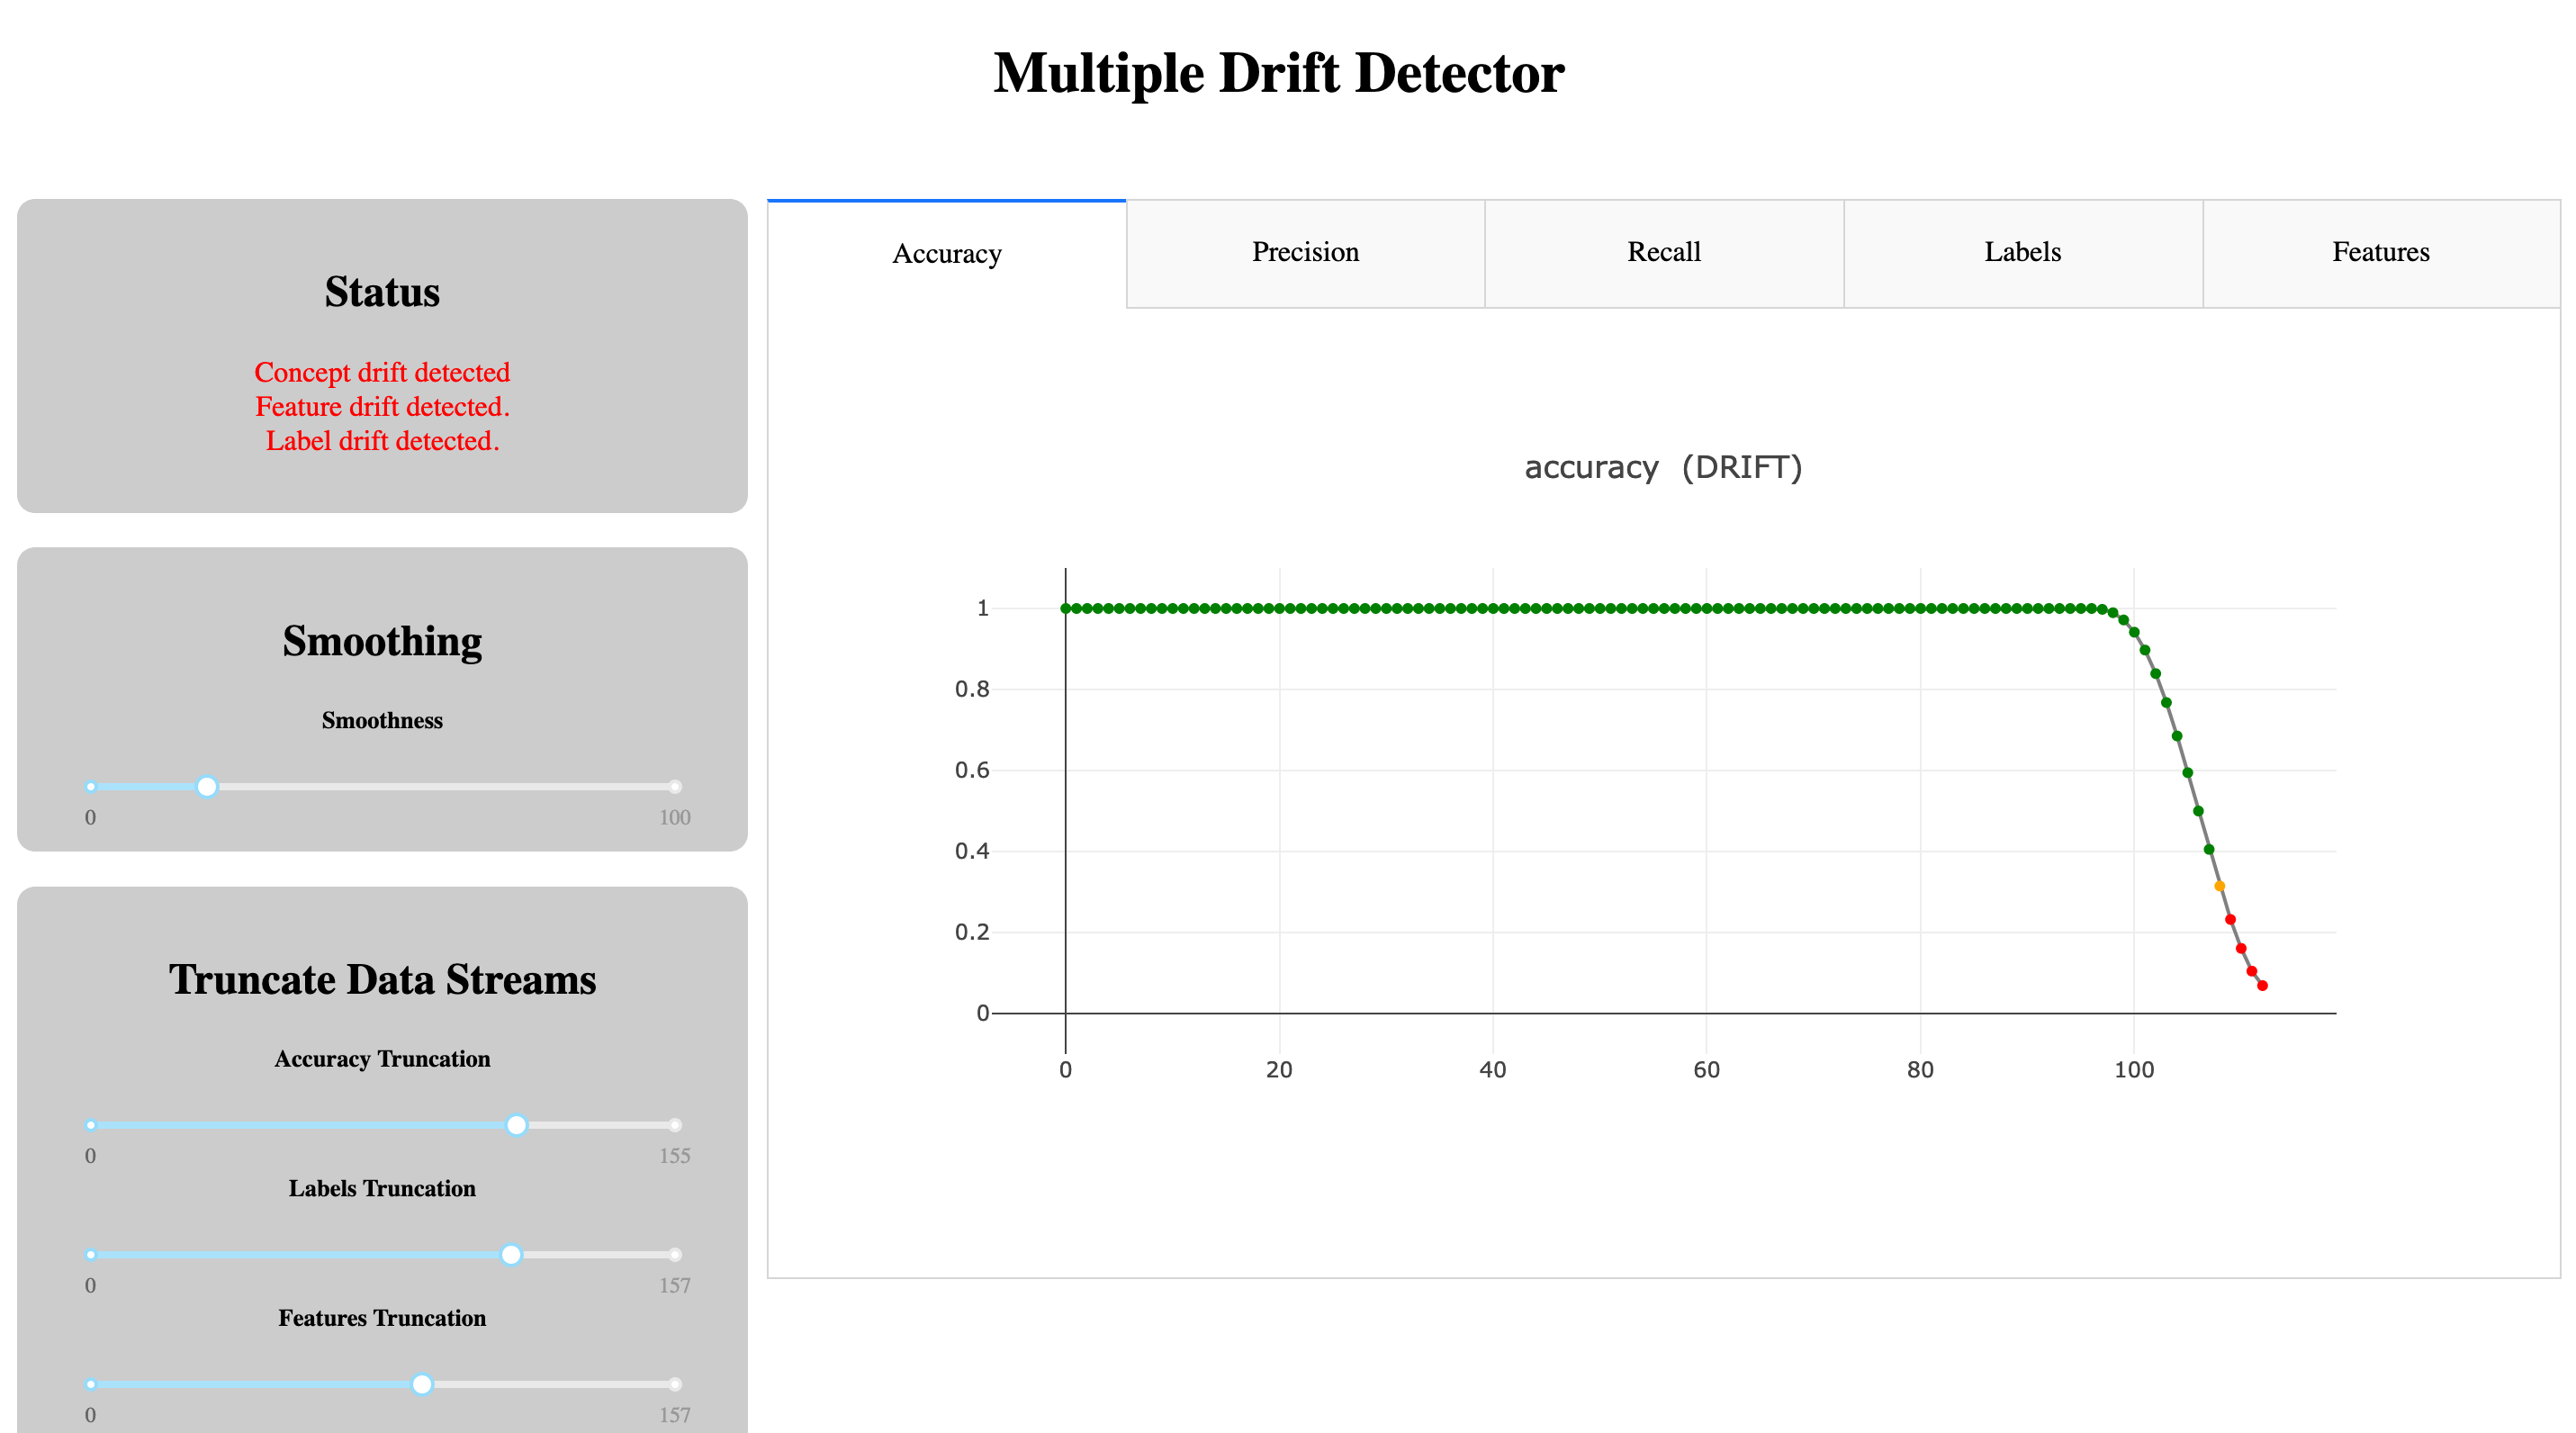
\includegraphics[width=\columnwidth]{images/dash_app.png}
    \caption{The graphical interface for multiple drift detector.}
    \label{fig:dash_app}
\end{figure}

%-------------------------------------------------------------------
% ILLUSTRATION
%-------------------------------------------------------------------

\section{Illustration} \label{mdd:illustration}

In this section we illustrate MDD framework using our GP referrals triage motivating example. We explore three drift scenarios, and describe how MDD will facilitate responding to the drift appropriately. 

\subsection{Scenario 1: Retrain}

The human expert commissioned to maintain the GP referrals triage decision support system receives a message from MDD indicating that model recall has decreased for priority 4, and precision has decreased for priority 3, as shown in Figure \ref{fig:scenario1}. Upon investigation, it turns out that a new study has been released showing that coronavirus is more dangerous than previously thought. Patients with this condition are now given priority 4 rather than priority 3. 

The expert responds by removing all referral documents from the dataset of patients with coronavirus from before the study was released. The model is retrained on the new dataset, and is redeployed.

\begin{figure}
    \centering
    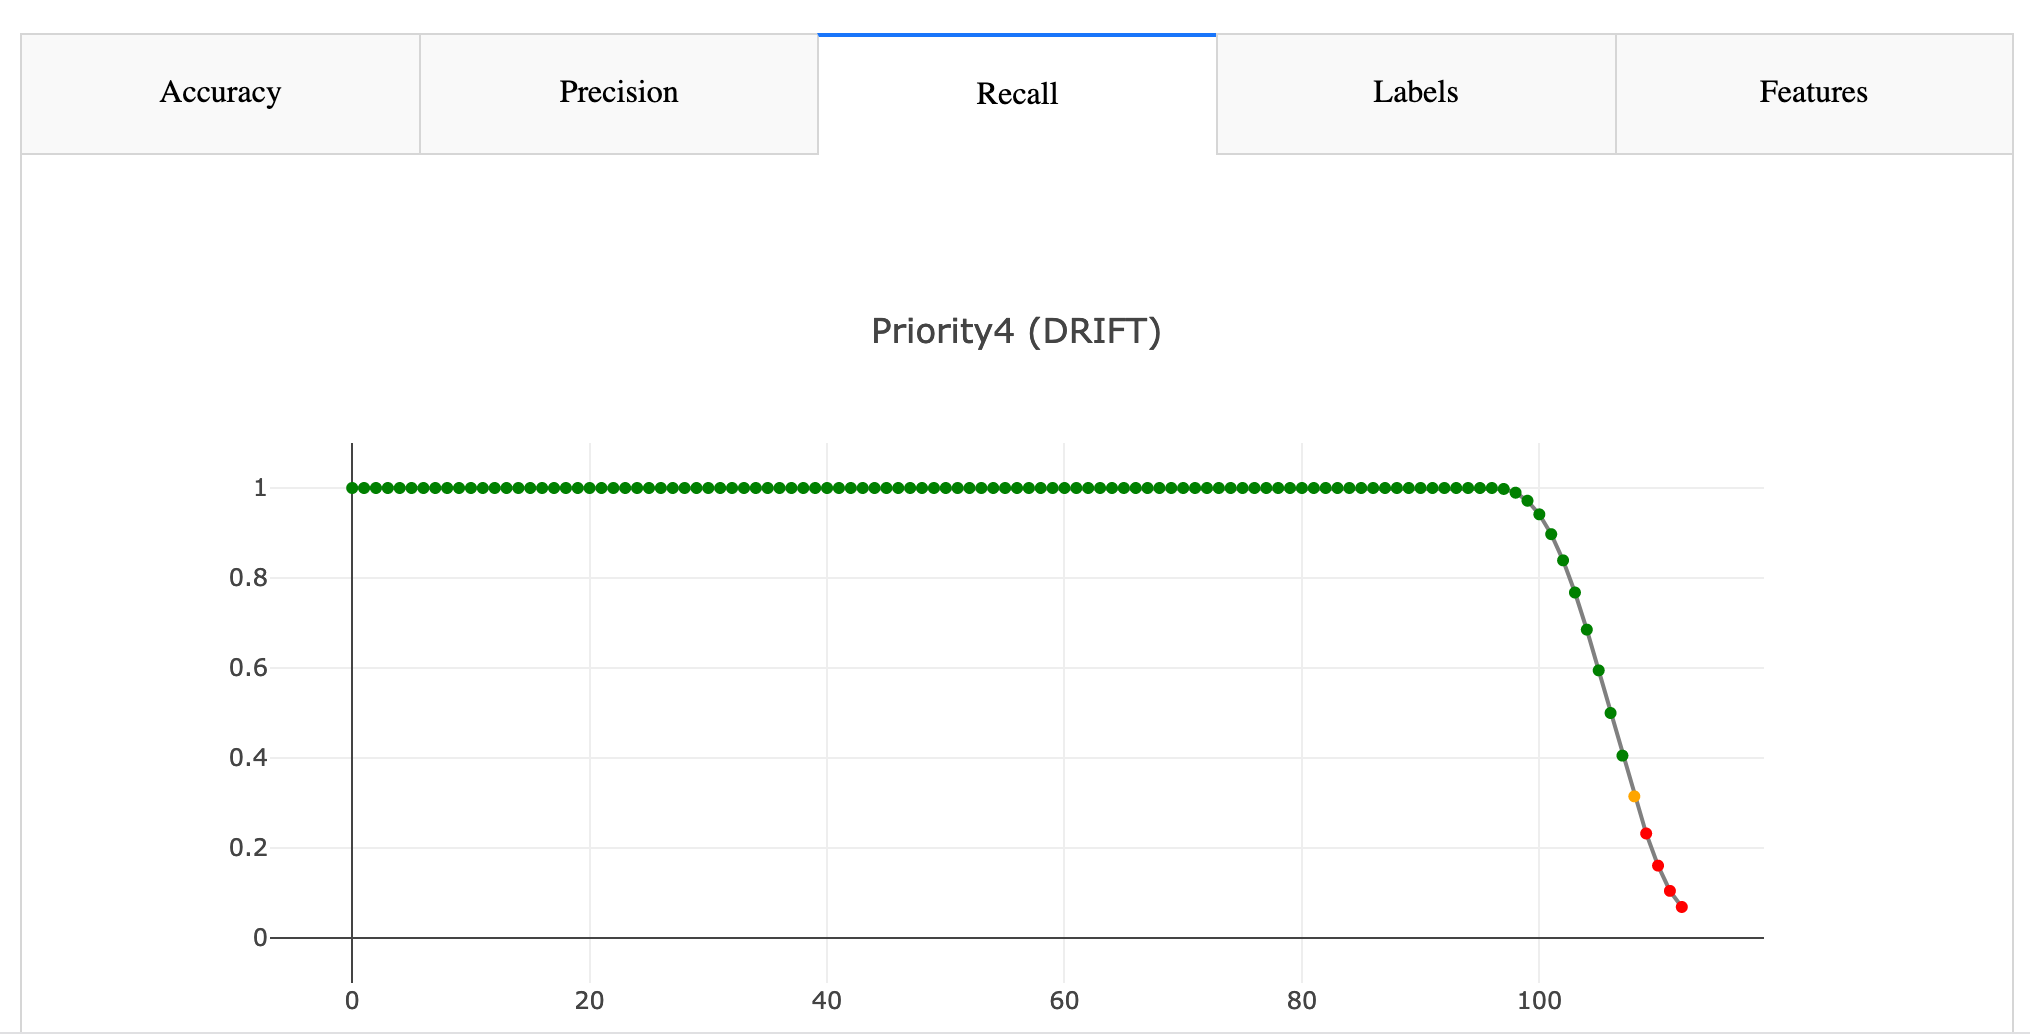
\includegraphics[width=\textwidth]{images/recall_p4.png}
    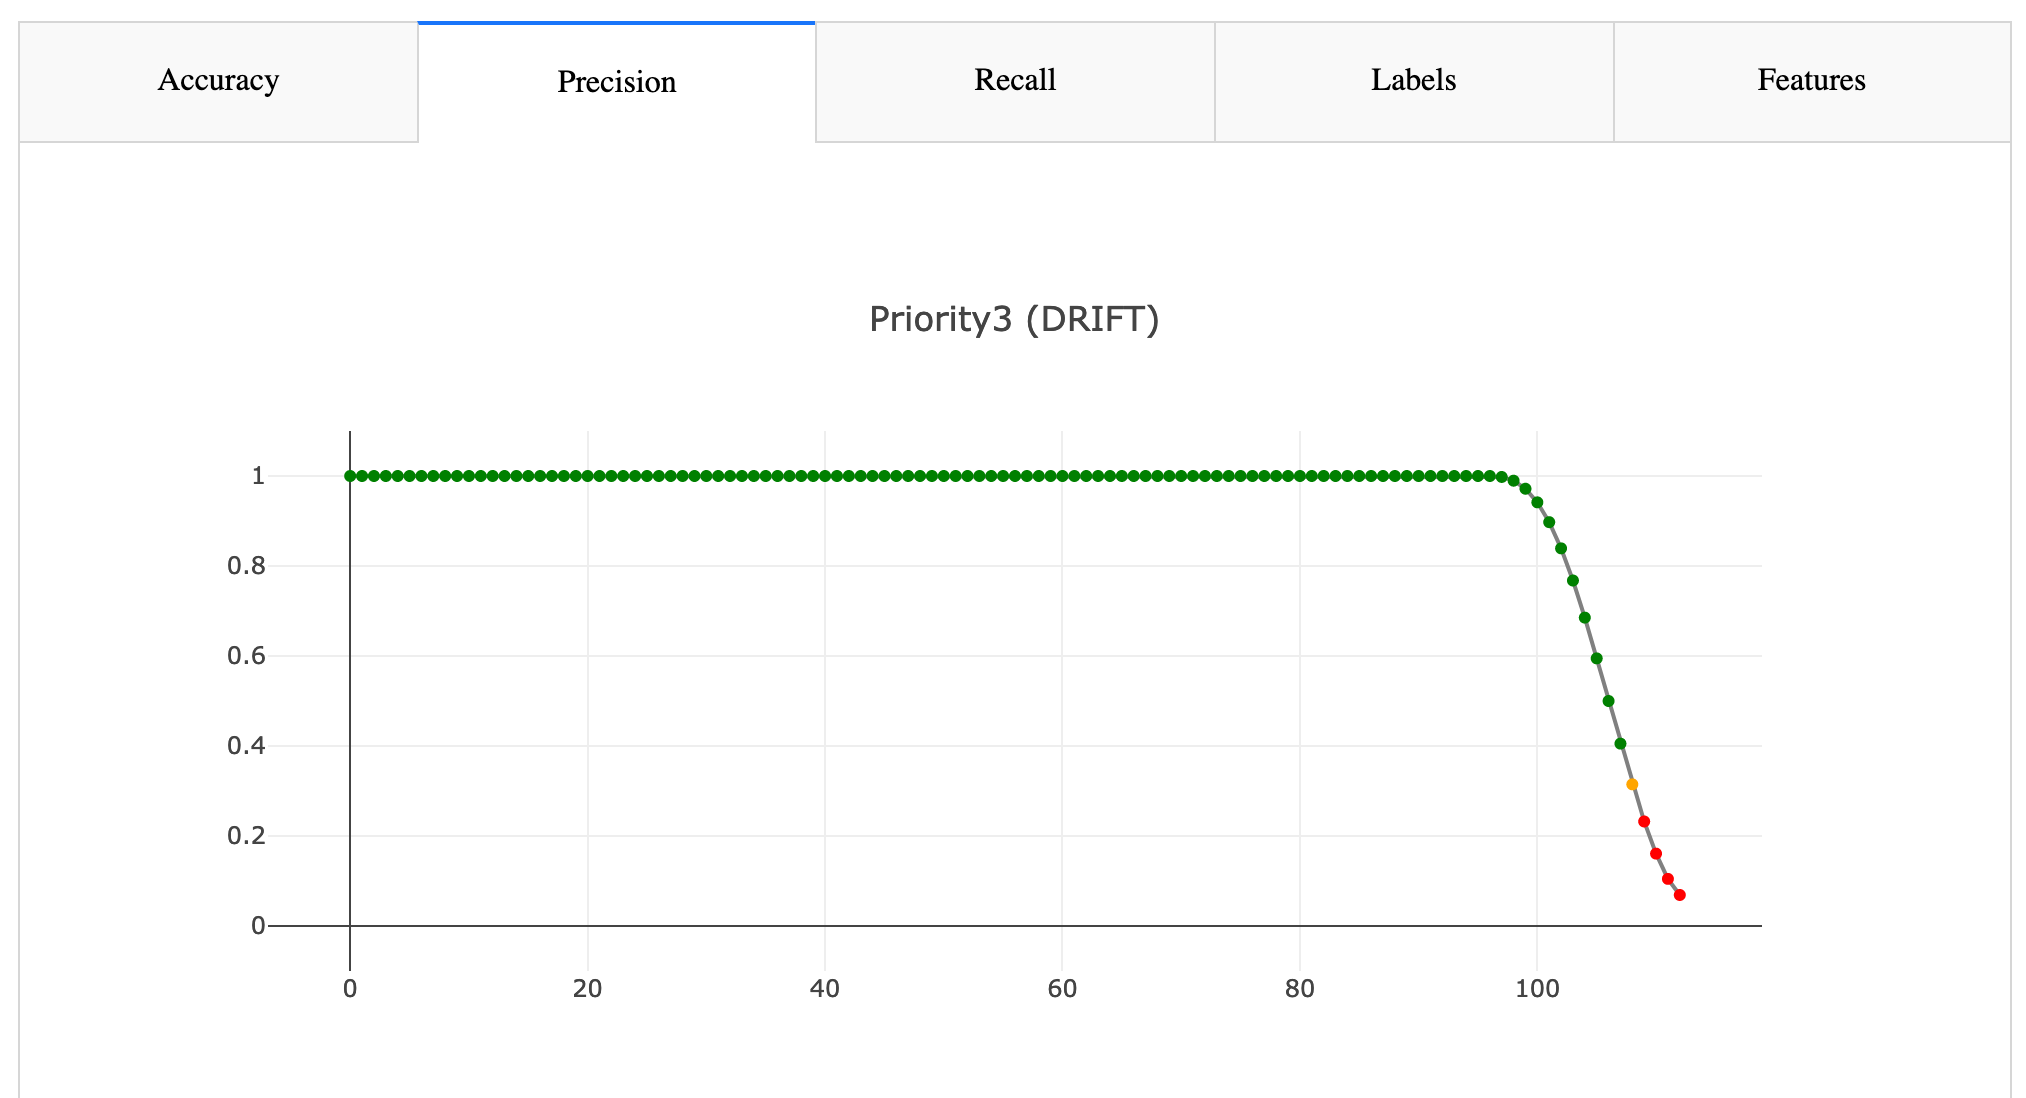
\includegraphics[width=\textwidth]{images/precision_p3.png}
    \caption{Scenario 1: Declining precision for triage priority 3 and declining recall for triage priority 4.}
    \label{fig:scenario1}
\end{figure}
 

\subsection{Scenario 2: No Action}

The human expert receives a message indicating that feature drift and label drift have both occurred. The expert inspects the feature time series in the graphical interface, and it appears that there has been an increase in referrals for patients with coronavirus, as shown in Figure \ref{fig:scenario2}. Because these instances are given priority 4, there has also been an increase in priority 4 labels, hence the label drift. Because the model has been trained on an adequate amount of referral documents which include coronavirus, it is able to correctly predict the priorities and this is correct behaviour so no action is required.

The expert checks in on model performance a week later when the clinicians have caught given priority labels to the referrals under the new distribution. The performance metrics haven't changed significantly, and the model was indeed adjusting to the change in distribution correctly.

\begin{figure}
    \centering
    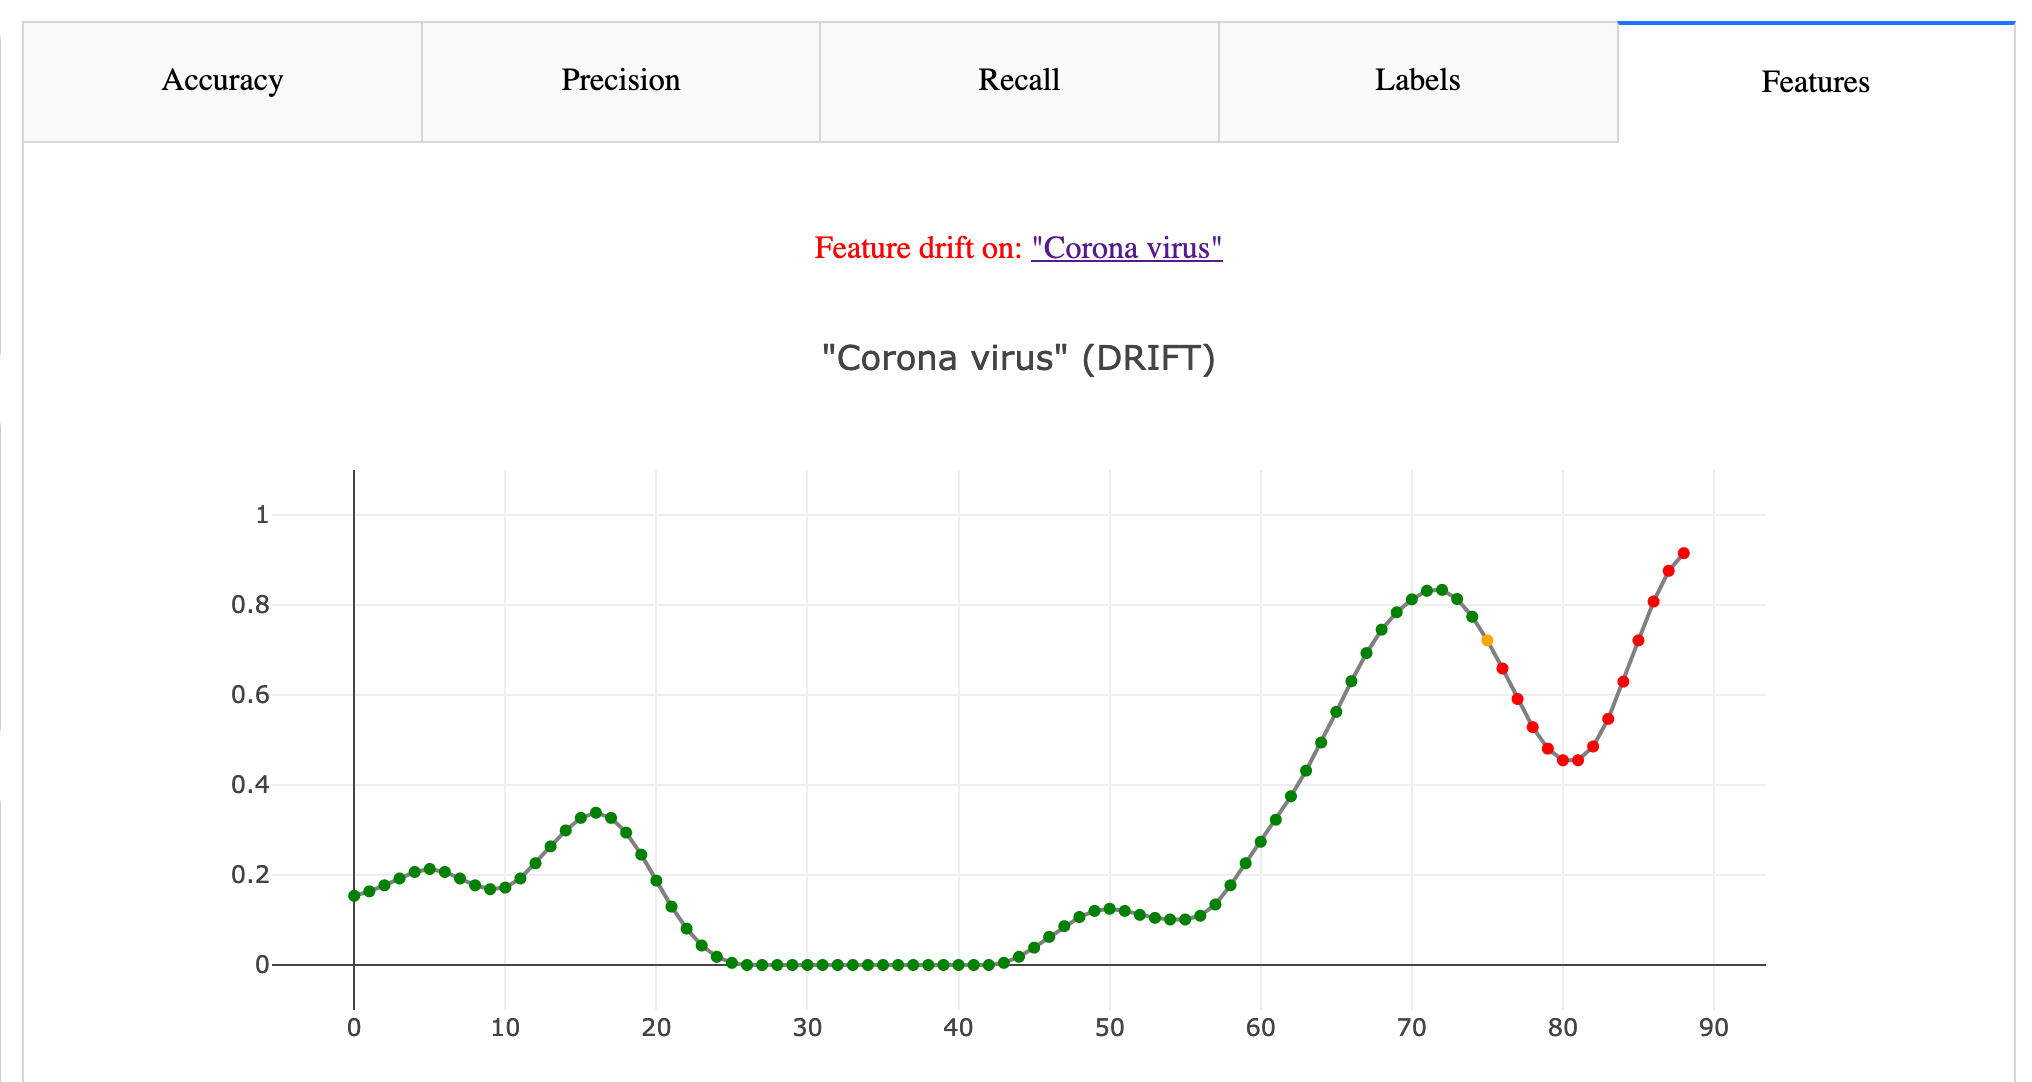
\includegraphics[width=\textwidth]{images/corona_virus.png}
    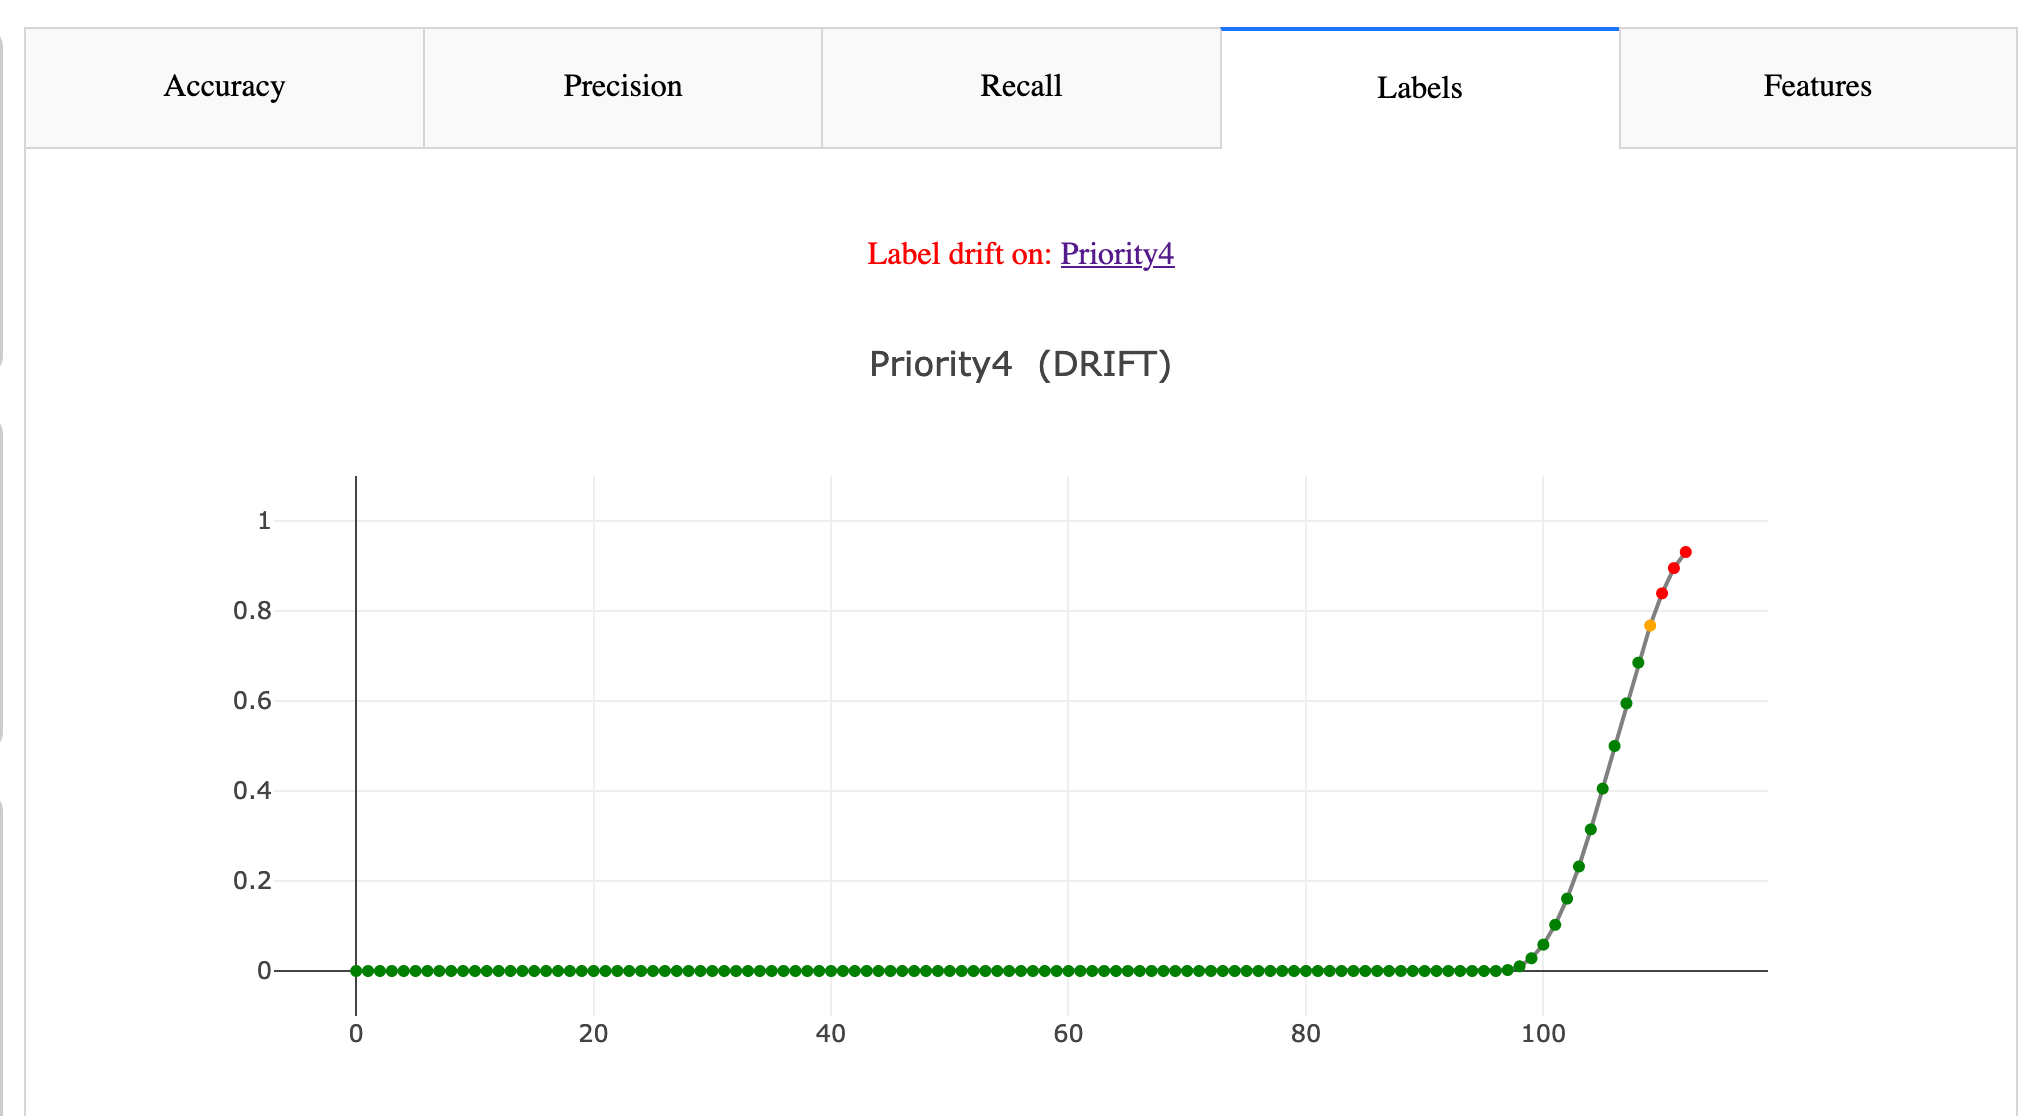
\includegraphics[width=\textwidth]{images/priority4.png}
    \caption{Scenario 2: Increase in the rate of triage priority 4 and increase in the rate of feature ``Corona virus".}
    \label{fig:scenario2}
\end{figure}


\subsection{Scenario 3: Recall}

The human expert receives a message indicating that feature drift has occurred. The expert inspects the feature time series in the graphical interface, and it appears that there has been an increase in referrals for patients with coronavirus, as shown in Figure \ref{fig:scenario3}. Because there were no coronavirus patients in the training data, the experts conclude that the model will be unable to make sensible triage predictions for this current wave of patients.These predictions are therefore clinically unsafe, and so should be withdrawn from the decision support system.

The expert therefore adds a rule to the decision support system stating that if a patient has coronavirus, the model should refrain from making a prediction, and annotate the referral as requiring a clinician to label it.
Once a sufficient dataset of labels for coronavirus patients has accumulated, the model is retrained to handle this new class of patient referral. 

\begin{figure}
    \centering
    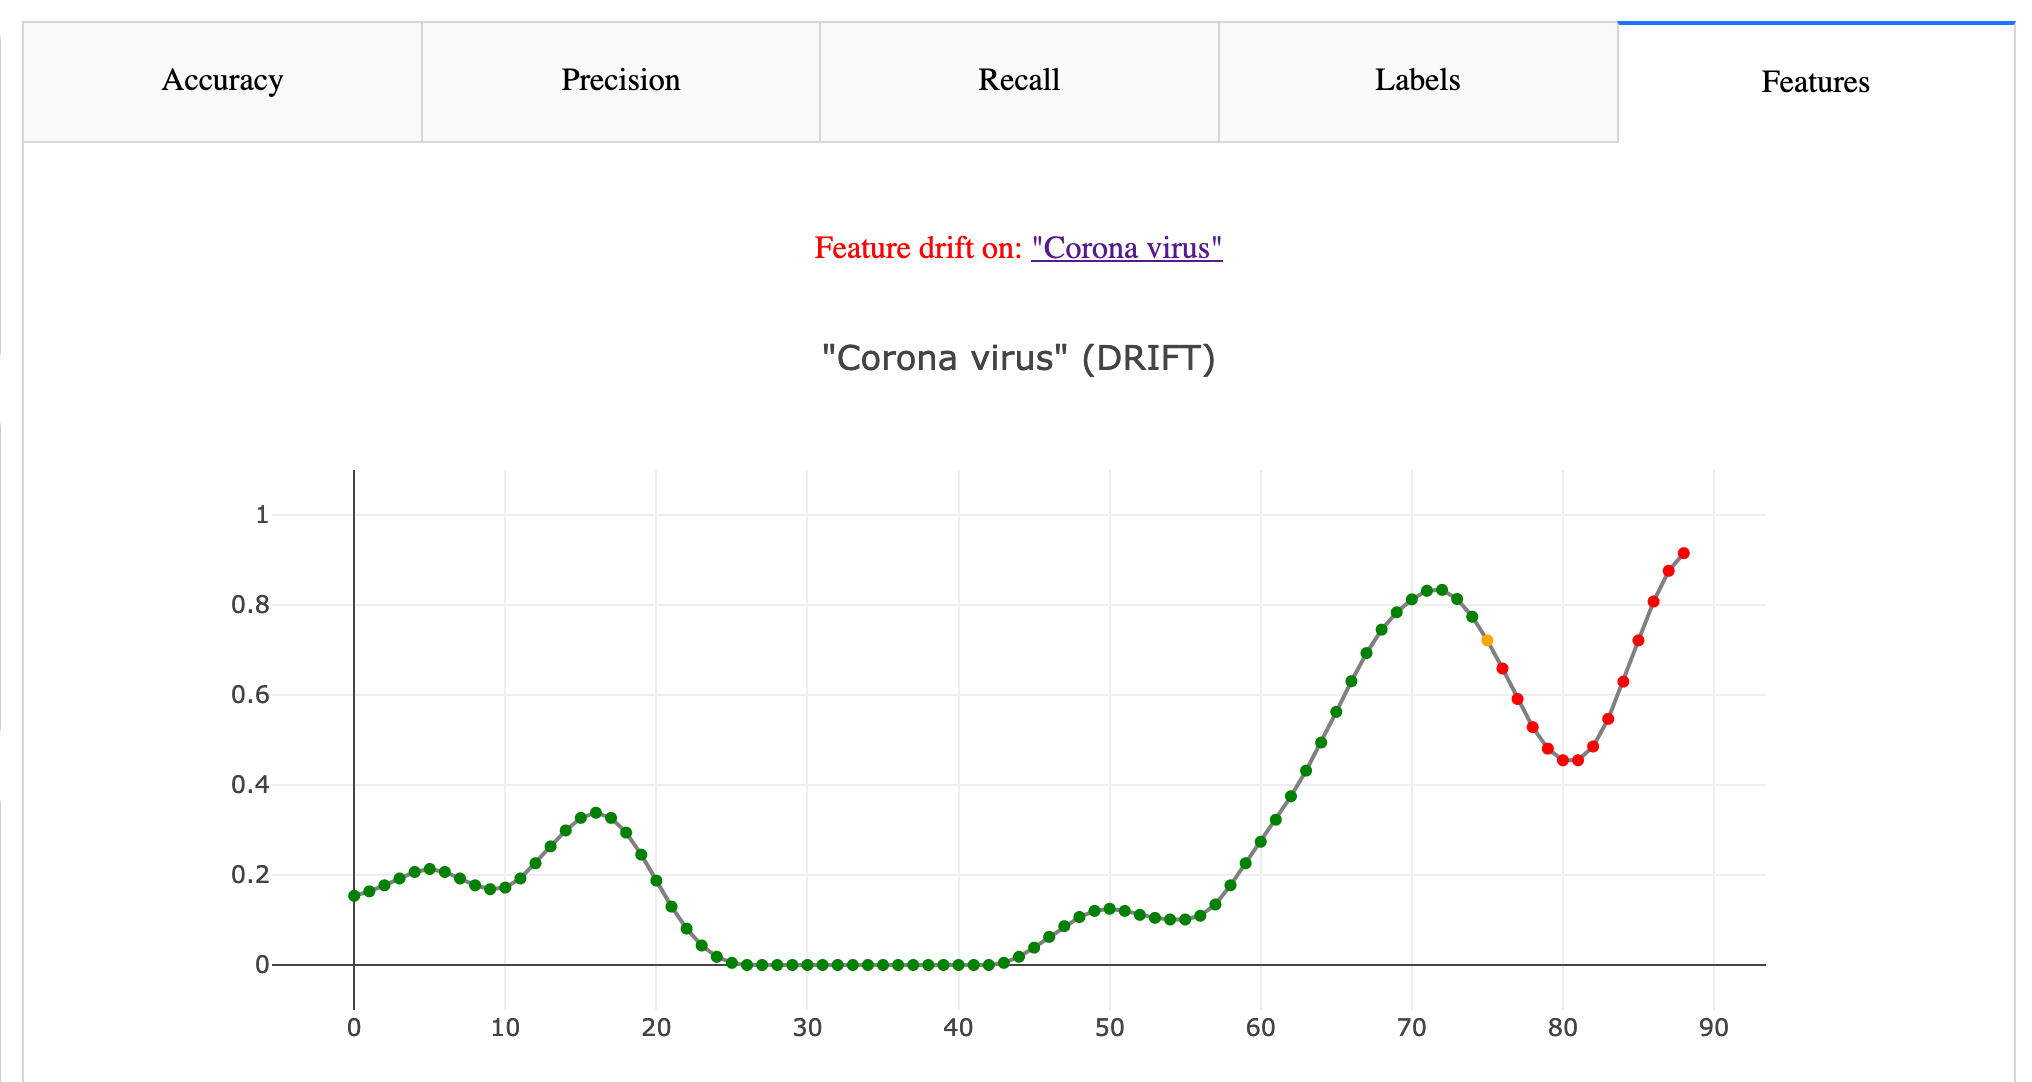
\includegraphics[width=\textwidth]{images/corona_virus.png}
    \caption{Scenario 3: Increase in the rate of feature ``Coronavirus" only.}
    \label{fig:scenario3}
\end{figure}


%-------------------------------------------------------------------
% CONCLUSION
%-------------------------------------------------------------------

\section{Conclusion} \label{mdd:conclusion}

In this chapter we introduced a framework for providing early warnings that a model requires retraining or recall, the multiple drift detector (MDD). MDD monitors the instance distribution, the label distribution, and model performance metrics for indicators of concept drift. We also present a graphical interface for visualising the evolution of the data stream and the state of MDD. 

In future work, we would like to validate that MDD works well in real applications by performing a user study.
